\documentclass[conference]{IEEEtran}
\IEEEoverridecommandlockouts

\usepackage{cite}
\usepackage{amsmath,amssymb,amsfonts}
\usepackage{graphicx}
\usepackage{textcomp}
\usepackage{xcolor}
\usepackage{listings}
\usepackage{booktabs}
\usepackage{url}
\usepackage{hyperref}
\usepackage{tikz}
\usetikzlibrary{arrows.meta, positioning, shapes.geometric}
\hypersetup{hidelinks}
\usepackage{placeins}
\usepackage{float}

\lstset{
  basicstyle=\ttfamily\footnotesize,
  breaklines=true,
  columns=fullflexible,
  showstringspaces=false,
  frame=single,
  rulecolor=\color{black!30}
}

\def\BibTeX{{\rm B\kern-.05em{\sc i\kern-.025em b}\kern-.08em
    T\kern-.1667em\lower.7ex\hbox{E}\kern-.125emX}}

\begin{document}

\title{A Low-Cost Two-Node IoT Gateway for Indoor Air Quality Monitoring with Co-Location Calibration and MQTT-TLS Telemetry}

\author{
\IEEEauthorblockN{
Pham Tan Thinh \quad Nguyen Huynh Thanh Phuc \quad Nguyen Dinh Thai Tue
}
\IEEEauthorblockA{
ECE-ICT, Vietnamese--German University, Binh Duong, Vietnam\\
Email: 10223067@student.vgu.edu.vn, 10223061@student.vgu.edu.vn, 10223071@student.vgu.edu.vn
}
}

\maketitle

\begin{abstract}
We present a low-cost indoor air quality monitoring node built on two ESP32-WROOM-32 microcontrollers in a sensor-to-gateway architecture. The sensor node samples Alphasense CO-B4 and NO\textsubscript{2}-B43F electrochemical sensors via an ADS1115 16-bit differential ADC, together with three temperature/humidity sensors (Sensirion SHT3x, DHT22, DHT11) for cross-sensor comparison. JSON-encoded measurements are forwarded over UART to a gateway node which publishes them to a Mosquitto broker over MQTT secured with TLS~1.3, where they are rendered on a custom Node-RED dashboard. The system was calibrated by co-location against an Aeroqual S500 reference instrument. After an initial warm-up calibration, a final one-hour co-location run was used to refine the electronic-zero offsets of the electrochemical channels. The final deployed firmware used a session-specific clean-air zero of $131.0$~mV for CO and a single-point NO\textsubscript{2} zero offset of $3.80$~mV while retaining the nominal sensitivity slopes. The end-to-end pipeline, including TLS authentication and live dashboard rendering, was verified.
\end{abstract}

\begin{IEEEkeywords}
Internet of Things, ESP32, air quality monitoring, electrochemical sensors, MQTT, TLS, Node-RED, co-location calibration.
\end{IEEEkeywords}

\section{Introduction}
Low-cost air quality sensors have become an active research area because regulatory-grade instruments are expensive and spatially sparse \cite{castell2017,mead2013}. Electrochemical (EC) sensors such as the Alphasense B4 series offer ppb-level sensitivity at a fraction of the cost of reference monitors, but require careful signal conditioning, calibration against a reference, and a robust telemetry path before their readings can be trusted.

This project implements a complete monitoring node addressing all three requirements. The contributions are: (i)~a clean sensor-to-gateway hardware architecture that isolates the analog signal chain from the wireless radio, (ii)~empirical calibration of the CO and NO\textsubscript{2} channels against an Aeroqual S500 reference, and (iii)~a secured telemetry stack using MQTT over TLS feeding a live web dashboard. The system was deployed and verified in the ECE Communication Networks laboratory at Vietnamese--German University.

\section{System Architecture}

\subsection{Hardware Overview}
The system uses two ESP32-WROOM-32 development boards in distinct roles:

\begin{itemize}
\item \textbf{Sensor node (Board A)}: 38-pin ESP32, handles all sensor I/O. WiFi is disabled to keep the analog supply rail clean.
\item \textbf{Gateway node (Board B)}: 30-pin ESP32, no sensors. Receives JSON over UART2 and publishes to MQTT over WiFi.
\end{itemize}

The split serves two purposes. First, electrochemical sensors are sensitive to power-rail noise; isolating WiFi RF bursts from the analog supply reduces baseline noise. Second, it cleanly separates concerns between sensing and networking, which is a common pattern in production IoT designs.

The sensor stack on Board A consists of:
\begin{itemize}
\item Sensirion SHT3x (I\textsuperscript{2}C @ 0x44) -- primary T/RH.
\item DHT22 and DHT11 (1-wire on GPIO 25 and 26) -- comparison T/RH.
\item ADS1115 (I\textsuperscript{2}C @ 0x48) -- 16-bit differential ADC for the gas sensors.
\item Alphasense CO-B4 on ISB (differential output to ADS1115 AIN0/AIN1).
\item Alphasense NO\textsubscript{2}-B43F on ISB (differential output to ADS1115 AIN2/AIN3).
\end{itemize}

\subsection{ADC Justification}
The ESP32's integrated 12-bit ADC has a least-significant-bit step of approximately $0.8$~mV across its 0--3.3~V range and exhibits non-linearity even after two-point calibration. Electrochemical sensor outputs at typical indoor concentrations are in the sub-millivolt range relative to a small baseline offset, which exceeds the practical resolution of the integrated ADC. The ADS1115, configured to a $\pm 0.512$~V full-scale range, provides approximately $16~\mu$V per LSB with true differential measurement, well matched to the signal.

\subsection{Voltage Domain Considerations}
The Alphasense ISB requires a 3.5--6.4~V supply and is powered from 5~V (VIN rail). Critically, the ISB output voltage at full scale can exceed the ADS1115's input absolute maximum of $V_{DD}+0.3$~V when the ADC is powered at 3.3~V. To avoid sensor-induced damage, the ADS1115 is powered from 5~V, raising its input tolerance ceiling to 5.3~V. The I\textsuperscript{2}C pull-ups remain on the 3.3~V rail, keeping bus logic levels safe for the ESP32 GPIOs.

A multimeter check was performed on each ISB output before connecting it to the ADC: each OP1/OP2 pin measured 0.2--0.6~V referenced to the common ground, confirming safe operation.

\subsection{Inter-Board Link}
The two boards communicate over UART2 at 115{,}200~baud:
\begin{itemize}
\item Board~A GPIO17 (TX2) $\rightarrow$ Board~B GPIO16 (RX2).
\item Common ground between the boards.
\end{itemize}
UART0 was deliberately avoided as it is shared with the USB-serial console and would conflict with flashing/monitoring. The protocol is one JSON line per measurement, newline-terminated.

\subsection{System Block Diagram}
Figure~\ref{fig:block_diagram} shows the implemented two-node architecture. Board~A performs all sensor acquisition and calibration, while Board~B acts as a network gateway. The separation is intentional: the analog electrochemical sensing chain is kept on the non-WiFi board to reduce interference from wireless transmission, while the gateway board handles WiFi, MQTT, and TLS communication.

\begin{figure*}[t]
\centering
\resizebox{0.95\textwidth}{!}{
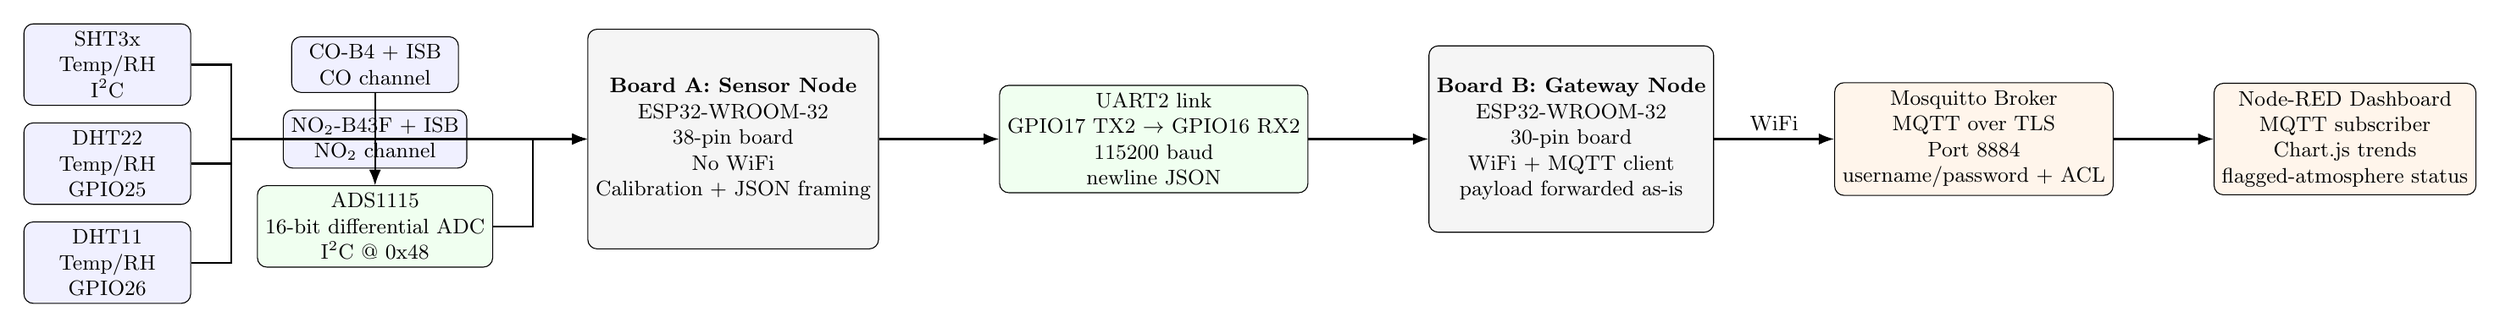
\begin{tikzpicture}[
    font=\small,
    block/.style={
        draw,
        rounded corners,
        minimum width=2.6cm,
        minimum height=1.0cm,
        align=center,
        fill=gray!8
    },
    sensor/.style={
        draw,
        rounded corners,
        minimum width=2.5cm,
        minimum height=0.8cm,
        align=center,
        fill=blue!6
    },
    process/.style={
        draw,
        rounded corners,
        minimum width=2.9cm,
        minimum height=1.0cm,
        align=center,
        fill=green!6
    },
    net/.style={
        draw,
        rounded corners,
        minimum width=2.9cm,
        minimum height=1.0cm,
        align=center,
        fill=orange!8
    },
    arrow/.style={-Latex, thick}
]

% Sensors
\node[sensor] (sht) {SHT3x\\Temp/RH\\I\textsuperscript{2}C};
\node[sensor, below=0.25cm of sht] (dht22) {DHT22\\Temp/RH\\GPIO25};
\node[sensor, below=0.25cm of dht22] (dht11) {DHT11\\Temp/RH\\GPIO26};

\node[sensor, right=1.5cm of sht] (co) {CO-B4 + ISB\\CO channel};
\node[sensor, below=0.25cm of co] (no2) {NO\textsubscript{2}-B43F + ISB\\NO\textsubscript{2} channel};
\node[process, below=0.25cm of no2] (ads) {ADS1115\\16-bit differential ADC\\I\textsuperscript{2}C @ 0x48};

% Board A
\node[block, right=1.8cm of no2, minimum width=3.6cm, minimum height=3.3cm] (boarda) {
\textbf{Board A: Sensor Node}\\
ESP32-WROOM-32\\
38-pin board\\
No WiFi\\
Calibration + JSON framing
};

% UART
\node[process, right=1.8cm of boarda] (uart) {
UART2 link\\
GPIO17 TX2 $\rightarrow$ GPIO16 RX2\\
115200 baud\\
newline JSON
};

% Board B
\node[block, right=1.8cm of uart, minimum width=3.6cm, minimum height=2.8cm] (boardb) {
\textbf{Board B: Gateway Node}\\
ESP32-WROOM-32\\
30-pin board\\
WiFi + MQTT client\\
payload forwarded as-is
};

% Network
\node[net, right=1.8cm of boardb] (broker) {
Mosquitto Broker\\
MQTT over TLS\\
Port 8884\\
username/password + ACL
};

\node[net, right=1.5cm of broker] (dash) {
Node-RED Dashboard\\
MQTT subscriber\\
Chart.js trends\\
flagged-atmosphere status
};

% Connections
\draw[arrow] (sht.east) -- ++(0.6,0) |- (boarda.west);
\draw[arrow] (dht22.east) -- ++(0.6,0) |- (boarda.west);
\draw[arrow] (dht11.east) -- ++(0.6,0) |- (boarda.west);

\draw[arrow] (co.south) -- (ads.north);
\draw[arrow] (no2.south) -- (ads.north);
\draw[arrow] (ads.east) -- ++(0.6,0) |- (boarda.west);

\draw[arrow] (boarda.east) -- (uart.west);
\draw[arrow] (uart.east) -- (boardb.west);
\draw[arrow] (boardb.east) -- node[above]{WiFi} (broker.west);
\draw[arrow] (broker.east) -- (dash.west);

\end{tikzpicture}
}

\vspace{0.8em}

\scriptsize
\begin{tabular}{@{}p{0.20\textwidth}p{0.24\textwidth}p{0.48\textwidth}@{}}
\toprule
Signal & Board / pin & Connection \\
\midrule
I\textsuperscript{2}C SDA & Board A GPIO21 & SHT3x SDA and ADS1115 SDA \\
I\textsuperscript{2}C SCL & Board A GPIO22 & SHT3x SCL and ADS1115 SCL \\
DHT22 data & Board A GPIO25 & DHT22 data line \\
DHT11 data & Board A GPIO26 & DHT11 data line \\
CO channel & ADS1115 AIN0/AIN1 & CO-B4 ISB OP1/OP2 differential pair \\
NO\textsubscript{2} channel & ADS1115 AIN2/AIN3 & NO\textsubscript{2}-B43F ISB OP1/OP2 differential pair \\
UART2 data path & A GPIO17 $\rightarrow$ B GPIO16 & Newline-terminated JSON stream at 115200 baud \\
Ground reference & Board A GND $\leftrightarrow$ Board B GND & Mandatory common reference \\
\bottomrule
\end{tabular}

\caption{Block diagram and key wiring summary of the implemented indoor air-quality monitoring system. Board~A performs sensor acquisition and gas calibration, while Board~B forwards the JSON payload to the MQTT-TLS telemetry stack.}
\label{fig:block_diagram}
\end{figure*}

\subsection{Physical Prototype}
Figure~\ref{fig:prototype_setup} shows the laboratory prototype used for the final demonstration. The sensor node consists of the 38-pin ESP32 board, the ADS1115 ADC, the SHT3x/DHT comparison sensors, and the two Alphasense electrochemical sensor channels. The 30-pin ESP32 board is used as a gateway node and is connected to the sensor node through UART2. This physical separation follows the system block diagram in Fig.~\ref{fig:block_diagram}: analog acquisition and calibration are performed on Board~A, while WiFi, MQTT, and TLS telemetry are handled by Board~B.



\begin{figure}[t]
\centering
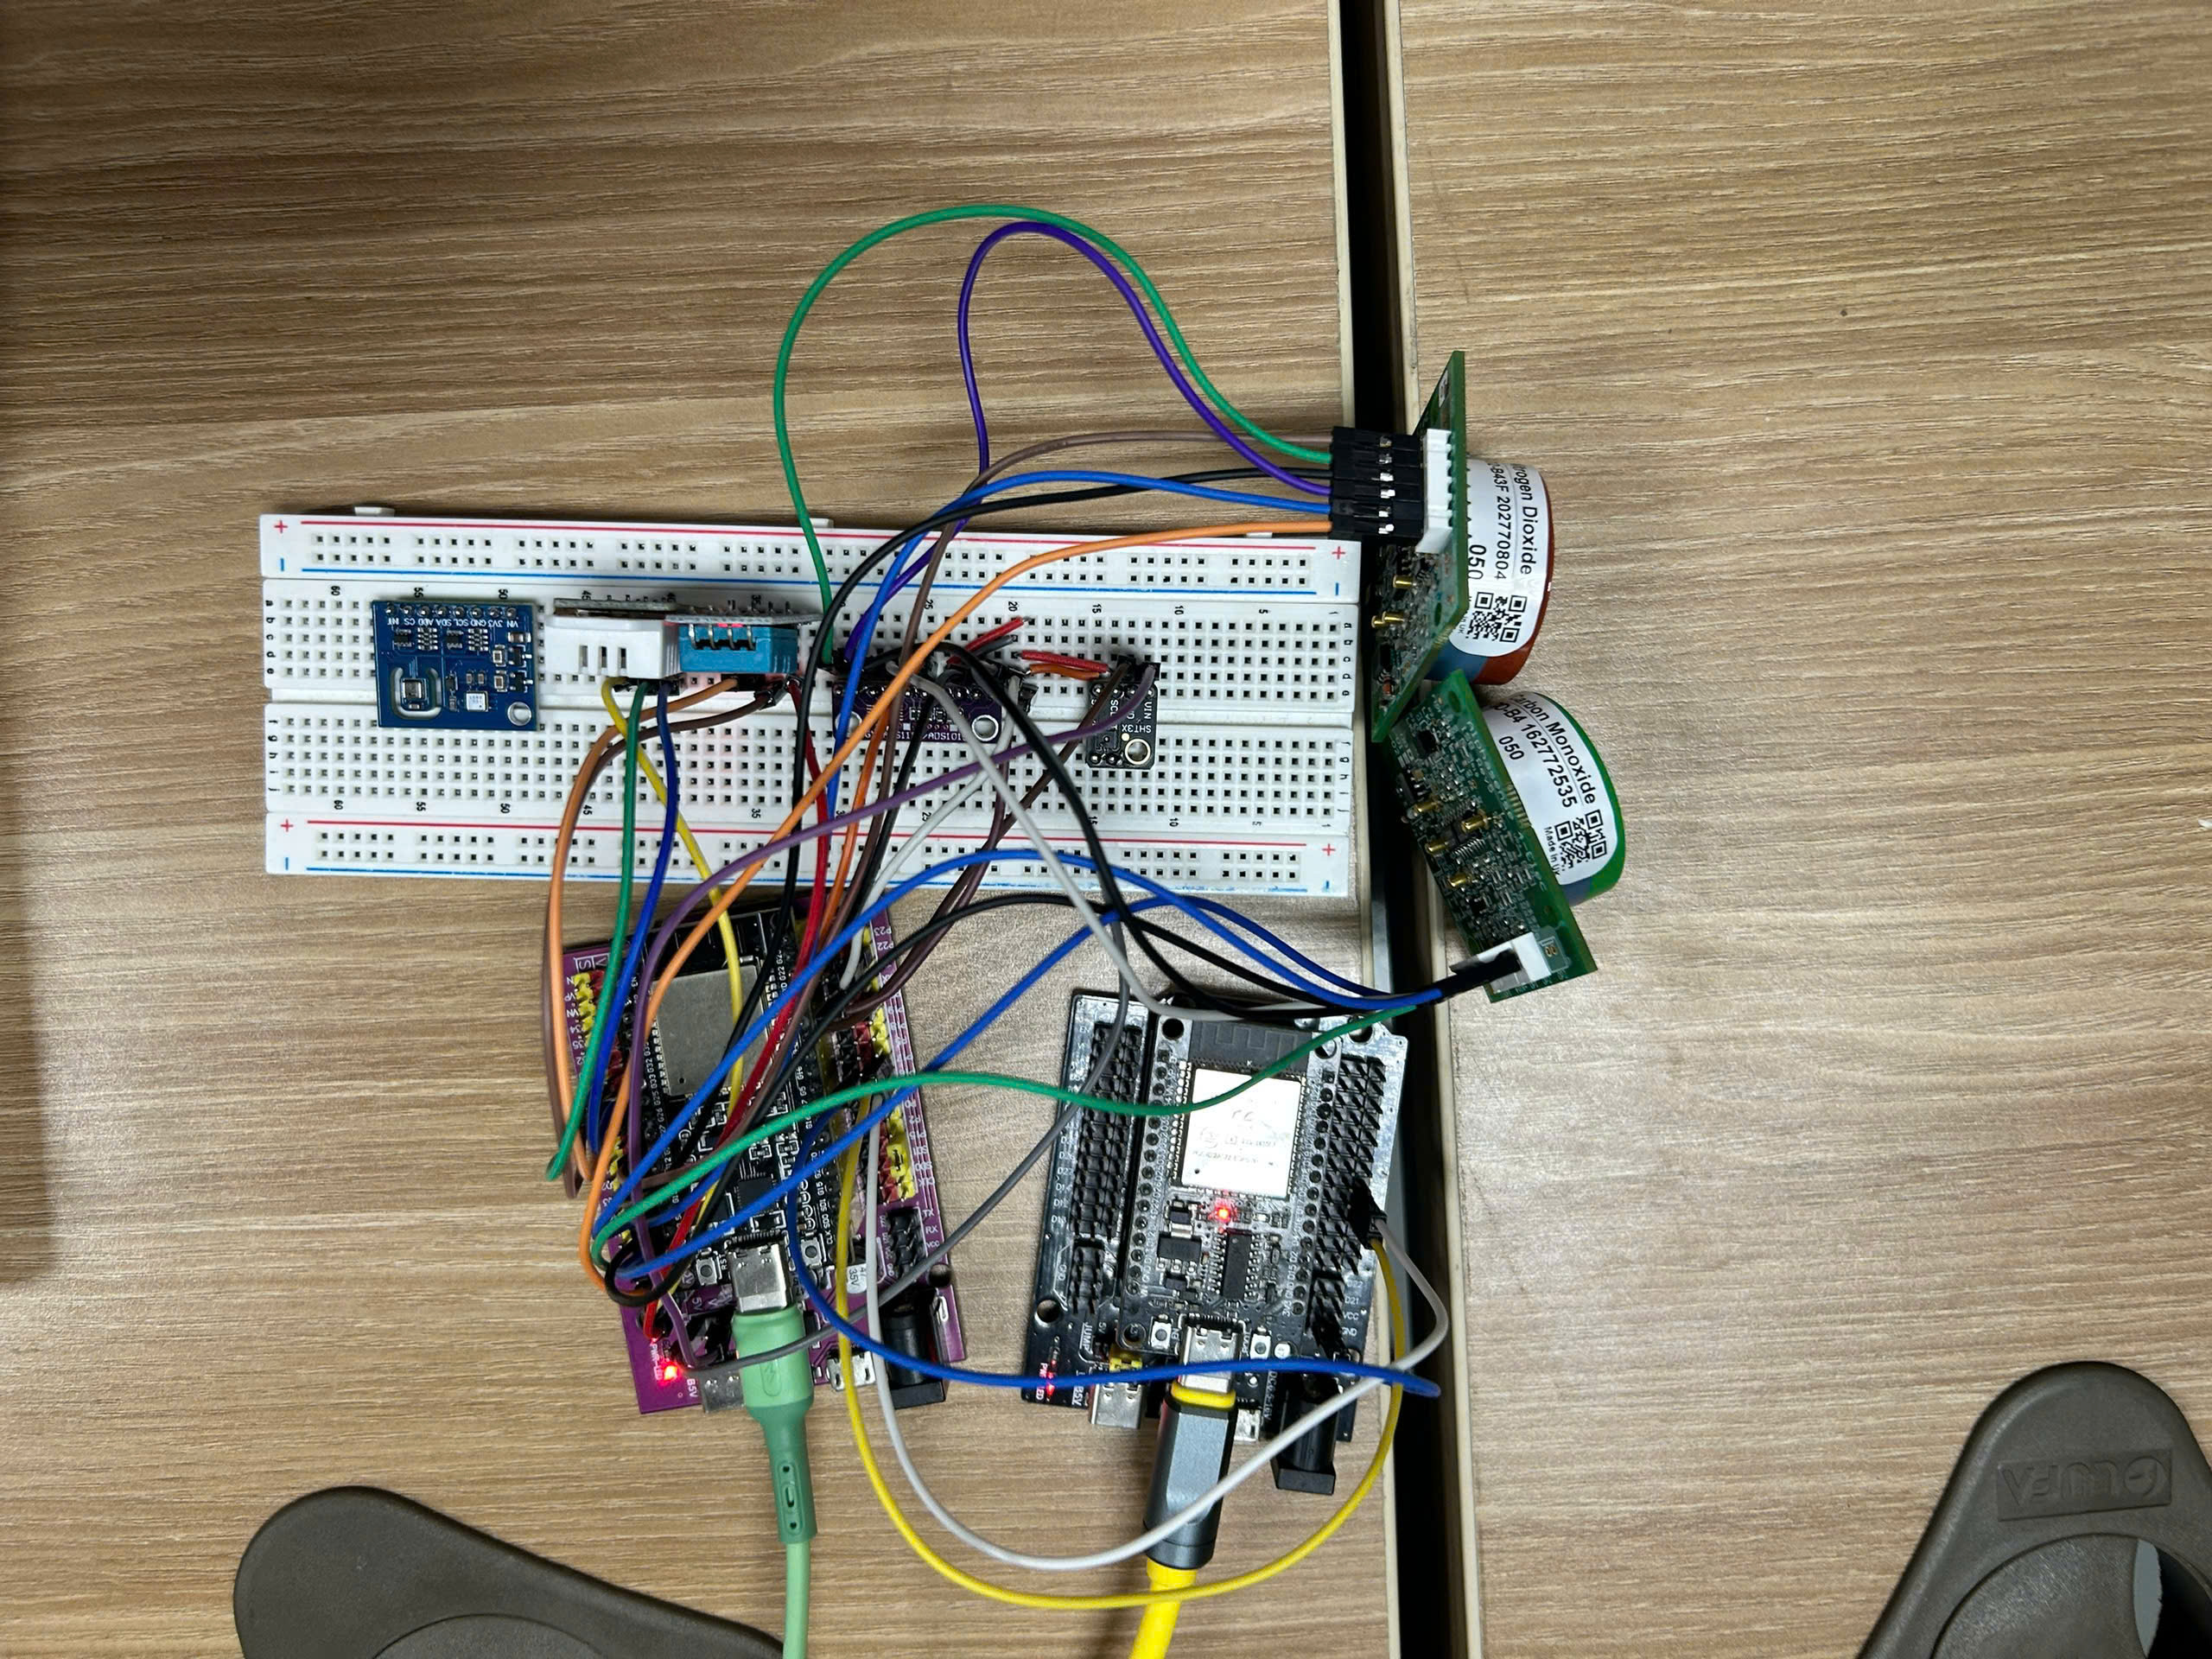
\includegraphics[width=\columnwidth]{prototype_setup.jpg}
\caption{Physical prototype of the two-node air-quality monitoring setup. Board~A performs sensor acquisition using the ADS1115 and environmental sensors, while Board~B forwards the JSON telemetry stream to the MQTT-TLS broker.}
\label{fig:prototype_setup}
\end{figure}

\section{Firmware}

\subsection{Sensor Node}
The sensor node firmware is implemented in ESP-IDF v6.0 and follows a single-task polling loop. Every $1$~s the firmware:
\begin{enumerate}
\item Reads SHT3x via I\textsuperscript{2}C with CRC verification.
\item Reads DHT22 and DHT11 via bit-banged 1-wire (each in a brief critical section to protect timing).
\item Triggers 16 successive ADS1115 conversions on differential channel 0 (CO) at 128 SPS, averaged.
\item Repeats step~3 on differential channel 1 (NO\textsubscript{2}).
\item Converts mV to ppb using the calibrated constants below.
\item Emits a JSON-encoded line over UART2 (binary path to the gateway) and a column-formatted line on UART0 (console for debugging).
\end{enumerate}

The ppb conversion is:
\begin{equation}
C_{\text{ppb}} = \frac{V_{\text{mV}} - V_{\text{zero}}}{S_{\text{mV/ppb}}}.
\label{eq:calib}
\end{equation}

Failed sensor reads (e.g., a dropped DHT frame) are emitted as JSON \texttt{null} rather than \texttt{NaN}, so downstream JSON parsers do not error.

\subsection{Gateway Node}
The gateway runs a minimal forward loop. It assembles bytes received on UART2 into newline-delimited lines, then republishes each line as the payload of an MQTT \texttt{PUBLISH} on topic \texttt{vgu/airquality/node1}. No transformation of the payload is performed; the gateway is intentionally a stateless bridge so all calibration logic resides in one place.

WiFi association uses the standard ESP-IDF \texttt{esp\_wifi} component. MQTT uses the \texttt{espressif/mqtt} managed component (relocated from the IDF core in v6.0) with the URI \texttt{mqtts://10.45.132.180:8884}, an embedded CA certificate, and username/password credentials.

\section{Telemetry, Security, and Dashboard}

\subsection{Broker and TLS}
Mosquitto~2.1.2 serves on port 8884 with a TLS-only listener. The CA was generated locally with OpenSSL; the server certificate's Subject Alternative Name includes both the laptop's LAN IP (\texttt{10.45.132.180}) and \texttt{localhost} so that both the ESP32 (LAN) and local test clients (loopback) can verify it. Anonymous access is disabled; both the gateway (\texttt{esp\_gateway}) and the dashboard (\texttt{nodered}) authenticate with username/password.

TLS~1.3 with the AES-256-GCM-SHA384 cipher suite is negotiated, as logged by Mosquitto on each gateway connection.

\subsection{Dashboard}
The dashboard runs in Node-RED with a single \texttt{ui\_template} node containing the full HTML/CSS/JavaScript layout. It subscribes to the MQTT topic, parses each JSON payload, and updates four metric cards (CO, NO\textsubscript{2}, Temperature, Humidity), a live Chart.js trend plot, a circular air quality indicator, and four sensor-status chips. Chart.js is served locally via Node-RED's \texttt{httpStatic} so the dashboard does not require Internet access at runtime. The circular air-quality indicator is computed from the gas channels only: CO is normalized to ppm for threshold comparison, NO\textsubscript{2} is evaluated in ppb, and the displayed status corresponds to the higher-severity result between the two gases. Temperature and humidity are shown as comfort/context measurements and do not directly raise the flagged-atmosphere state.


\subsection{Flagged Atmosphere Indicator}
The dashboard includes a threshold-based flagged-atmosphere indicator for laboratory interpretation of the gas channels. This indicator is not presented as a certified safety alarm or a regulatory compliance measurement; it is a dashboard warning aid for the demonstrated indoor monitoring setup. Temperature and humidity are intentionally excluded from this gas-severity decision and are shown separately as environmental context.

Table~\ref{tab:airquality_thresholds} summarizes the thresholds used by the dashboard. CO is evaluated in ppm because CO exposure guidance is commonly expressed in ppm, whereas NO\textsubscript{2} is evaluated in ppb because indoor and ambient NO\textsubscript{2} levels are normally interpreted at ppb-scale concentrations. Since the sensor firmware reports both gas concentrations in ppb, CO is normalized before classification according to
\begin{equation}
C_{\mathrm{CO,ppm}} = \frac{C_{\mathrm{CO,ppb}}}{1000},
\label{eq:co_ppb_to_ppm}
\end{equation}
while NO\textsubscript{2} is used directly as $C_{\mathrm{NO_2,ppb}}$. Conversely, if a future payload provides CO in ppm or NO\textsubscript{2} in ppm, the dashboard converts CO to a ppb display value using $C_{\mathrm{CO,ppb}}=1000C_{\mathrm{CO,ppm}}$ and NO\textsubscript{2} to ppb using $C_{\mathrm{NO_2,ppb}}=1000C_{\mathrm{NO_2,ppm}}$.

\begin{table}[t]
\centering
\caption{Dashboard threshold ranges for the flagged-atmosphere indicator.}
\label{tab:airquality_thresholds}
\scriptsize
\begin{tabular}{@{}lllp{0.25\columnwidth}@{}}
\toprule
Gas & Unit & Range & Status \\
\midrule
CO & ppm & 0--5 & Good \\
CO & ppm & $>5$--9 & Elevated \\
CO & ppm & $>9$--35 & Warning \\
CO & ppm & $>35$ & Alert \\
NO\textsubscript{2} & ppb & 0--21 & Good \\
NO\textsubscript{2} & ppb & $>21$--53 & Elevated \\
NO\textsubscript{2} & ppb & $>53$--106 & Warning \\
NO\textsubscript{2} & ppb & $>106$ & Alert \\
\bottomrule
\end{tabular}
\end{table}

The overall flagged-atmosphere state is computed as the worse of the two gas-channel severities using the ordering Good $<$ Elevated $<$ Warning $<$ Alert. For example, CO~=~365~ppb is first converted to 0.365~ppm and therefore remains in the Good range, while NO\textsubscript{2}~=~40~ppb falls in the Elevated range according to Table~\ref{tab:airquality_thresholds}. In that case the overall indicator is Elevated because it takes the higher-severity result between CO and NO\textsubscript{2}.

\subsection{TLS Verification}
To verify that TLS provides actual confidentiality and is enforced, three checks were performed:
\begin{itemize}
\item \textbf{Packet capture}: \texttt{tcpdump} on port 1883 (plaintext) showed JSON payloads in cleartext; on 8883/8884 (TLS) only encrypted bytes.
\item \textbf{Handshake inspection}: \texttt{openssl s\_client} returned \texttt{Verify return code: 0 (ok)} with the configured CA.
\item \textbf{Negative tests}: A plaintext client connecting to the TLS port was refused; a TLS client without the CA failed certificate verification.
\end{itemize}

\subsection{Pseudo-Attack Benchmark}
As an additional benchmark, a local pseudo-attack script (\texttt{mqtt\_tls\_benchmark.py}) was executed against the Mosquitto listener on \texttt{localhost:8884}. The benchmark did not attempt destructive activity; instead, it exercised the expected protection boundaries of the MQTT-TLS deployment: plaintext rejection on the TLS port, certificate and hostname verification, credential enforcement, ACL enforcement, and a replay/freshness limitation check. The test environment remained connected to the live sensor gateway during execution, so two message-content matching subtests were affected by normal telemetry published on the same topic.

\begin{table}[t]
\centering
\caption{Pseudo-attack benchmark against the MQTT-TLS broker.}
\label{tab:tls_benchmark}
\scriptsize
\setlength{\tabcolsep}{2.5pt}
\renewcommand{\arraystretch}{0.92}
\begin{tabular}{@{}p{0.38\columnwidth}p{0.15\columnwidth}p{0.39\columnwidth}@{}}
\toprule
Check & Result & Evidence / interpretation \\
\midrule
Tools and CA present & Pass & Test environment ready \\
TCP port 8884 reachable & Pass & TLS listener reachable \\
Plaintext to TLS port & Pass & Connection rejected \\
Trusted TLS handshake & Pass & TLS~1.3 / AES-256-GCM \\
Wrong hostname & Pass & Certificate verification failed \\
Missing credentials & Pass & Not authorized \\
Wrong password & Pass & Not authorized \\
Gateway publish path & Inconcl. & Live telemetry arrived first \\
Node-RED publish attempt & Pass & ACL blocked write access \\
Gateway subscribe attempt & Pass & ACL blocked read access \\
Replay/freshness check & Partial & Duplicate accepted; freshness missing \\
\bottomrule
\end{tabular}
\end{table}

Overall, 8 of the 10 automated checks passed directly. The two non-passing checks were not observed authentication or TLS failures: in both cases, \texttt{mosquitto\_sub} received a valid live sensor message before the benchmark payload because the ESP32 gateway was simultaneously publishing to \texttt{vgu/airquality/node1}. A cleaner rerun would isolate the benchmark on a temporary topic or temporarily disconnect the live gateway. This additional rerun was not performed because the lab access window was limited and the devices/components had to remain in the laboratory after the session. The result is therefore interpreted conservatively: the TLS, certificate verification, authentication, and ACL controls were demonstrated, while exact payload-matching and replay evaluation were left as future refinement.

The replay check also highlights a useful security boundary. TLS protects the confidentiality and authenticity of the transport channel, but it does not by itself provide application-layer freshness. An authenticated publisher can still send a syntactically valid duplicate JSON message. A future implementation should add a sequence number or timestamp field at the sensor node and reject stale or repeated messages at the dashboard or broker-side processing layer.

\section{Calibration Methodology}

\subsection{Approach}
The Alphasense ISBs in our lab inventory were unaccompanied by their factory calibration certificates. Nominal datasheet sensitivities were therefore used as starting values, and the calibration was refined by co-location with an Aeroqual S500 reference monitor. The CO-B4 datasheet specifies a sensitivity range of 420--650~nA/ppm, and the NO\textsubscript{2}-B43F datasheet specifies $-200$ to $-650$~nA/ppm. Combined with typical ISB transimpedance, these yield approximate mV/ppb values of $+0.35$ for CO and $-0.25$ for NO\textsubscript{2}.

The sensor was first co-located with the Aeroqual S500 in the ECE lab during warm-up to obtain preliminary electronic-zero estimates. Because electrochemical sensors exhibit baseline settling after power-up, a second one-hour co-location run was then performed after the system had stabilized further. Prototype readings were logged at approximately 1.4~s intervals through the ESP-IDF serial monitor, while Aeroqual values were extracted manually from a camera recording because direct digital export from the S500 was unavailable. The final calibration constants reported in this paper correspond to the deployed firmware used during the final validation run.

\subsection{Calibration Refinement}
The calibration was refined in two stages. The first stage provided preliminary offsets during sensor warm-up. The second stage used the final one-hour co-location run, after the electrochemical channels had stabilized more closely to the Aeroqual reference. Only the zero offsets were updated; the sensitivity slopes were not refitted because the co-location data contained a single stable concentration region rather than multiple controlled gas concentrations.

\begin{table}[t]
\centering
\caption{Final deployed calibration constants used in the validation run.}
\label{tab:final_calibration}
\scriptsize
\begin{tabular}{@{}llll@{}}
\toprule
Channel & Sensitivity & Final zero & Basis \\
\midrule
CO & $+0.350$ mV/ppb & $131.0$ mV & Clean-air baseline \\
NO\textsubscript{2} & $-0.250$ mV/ppb & $3.80$ mV & S500 one-hour anchor \\
\bottomrule
\end{tabular}
\end{table}

\subsection{Statistics Over the Co-Location Window}
Table~\ref{tab:colocstats} summarizes the measured values. The full log contains $n=1306$ samples spanning approximately 30~minutes.

\begin{table}[t]
\centering
\caption{Final one-hour co-location statistics after one-minute median quantization. Aeroqual S500 readings were logged manually at change points and expanded as a step-wise reference signal.}
\label{tab:colocstats}
\scriptsize
\setlength{\tabcolsep}{3pt}
\renewcommand{\arraystretch}{0.95}
\begin{tabular}{@{}p{0.42\columnwidth}rrr@{}}
\toprule
Quantity & Mean & Std. & Range \\
\midrule
Prototype CO ($V_{\text{mV}}$) & $96.15$ & $5.72$ & 88.94--108.11 \\
Prototype NO\textsubscript{2} ($V_{\text{mV}}$) & $-6.20$ & $0.25$ & $-6.60$--$-5.42$ \\
Prototype NO\textsubscript{2} (ppb) & $39.98$ & $0.98$ & 36.86--41.59 \\
S500 NO\textsubscript{2} (ppb) & $40.97$ & $1.19$ & 38--44 \\
Prototype CO (ppm) & $0.00$ & $0.00$ & 0.00--0.00 \\
S500 CO (ppm) & $0.00$ & $0.00$ & 0.00--0.00 \\
\bottomrule
\end{tabular}
\end{table}

\subsection{CO Calibration}
The laboratory contained no combustion source, and the Aeroqual S500 CO channel remained approximately at zero during the co-location run. Therefore, the CO channel was treated as a clean-air baseline calibration rather than a span calibration. The final deployed firmware used
\begin{align*}
S_{\text{CO}}      &= +0.350~\text{mV/ppb} \quad\text{(nominal)} \\
V_{\text{zero,CO}} &= 131.0~\text{mV} \quad\text{(session clean-air baseline)}.
\end{align*}
The CO concentration was then computed as
\[
C_{\text{CO,ppb}} = \frac{V_{\text{CO,mV}} - 131.0}{0.350}.
\]
This procedure forces the settled clean-air output to approximately 0~ppb, which is appropriate for the indoor laboratory validation. However, because no controlled CO source was available, the CO slope was not experimentally verified.

\subsection{NO\textsubscript{2} Calibration}
During the final one-hour co-location run, the Aeroqual S500 NO\textsubscript{2} reading stabilized around $0.039$--$0.041$~ppm, equivalent to approximately $39$--$41$~ppb. The prototype NO\textsubscript{2} channel produced a stable filtered differential-voltage cluster in the same period. Since only one concentration region was available, a full two-point regression was not possible. The sensitivity was therefore retained at the nominal value, and only the electronic-zero offset was updated:
\begin{align*}
S_{\text{NO}_2}      &= -0.250~\text{mV/ppb} \quad\text{(nominal)} \\
V_{\text{zero,NO}_2} &= 3.80~\text{mV}.
\end{align*}
The final NO\textsubscript{2} concentration was computed as
\[
C_{\text{NO}_2,\text{ppb}} =
\frac{V_{\text{NO}_2,\text{mV}} - 3.80}{-0.250}.
\]
For example, a filtered NO\textsubscript{2} voltage of approximately $-6.20$~mV corresponds to $40.0$~ppb, while $-6.45$~mV corresponds to approximately $41.0$~ppb. This matches the stabilized Aeroqual range during the final validation run.

\subsection{Limitations}
\label{ssec:limitations}
Two limitations of this calibration are stated honestly:
\begin{enumerate}
\item The S500's proprietary SC09-FX export cable was unavailable, so reference readings were logged manually rather than streamed. This reduces sample density on the reference side but does not affect the anchor point, which is robust to averaging because the S500 reading was stable across the window.
\item Both instruments observed a single stable concentration cluster. The applied calibration therefore corrects the offset (electronic zero) but cannot refine the slope (sensitivity) from this data. A full two-point span calibration would require controlled exposure to a known concentration (e.g., gas-cylinder reference or outdoor co-location with significant traffic-source NO\textsubscript{2}) and is identified as future work.
\end{enumerate}

These limitations are consistent with field-deployment practice for low-cost EC sensors in stable indoor environments \cite{castell2017,mead2013}.

\section{Results}

\subsection{Sensor Comparison}
With the three T/RH sensors deployed in parallel, their readings during the final co-location window are summarized in Table~\ref{tab:trh}. SHT3x reported the most stable and highest-resolution values; DHT22 tracked SHT3x closely with a slightly higher RH bias; DHT11 showed a noticeable temperature bias and lower resolution, consistent with its $\pm 2$\,\textdegree C / $\pm 5$\,\%RH datasheet specification.

\begin{table}[t]
\centering
\caption{Temperature and humidity sensor comparison over the final co-location window.}
\label{tab:trh}
\begin{tabular}{lrrr}
\toprule
Sensor & Mean T (\textdegree C) & Mean RH (\%) & Datasheet acc. \\
\midrule
SHT3x  & $\approx 26.3$ & $\approx 60.3$ & $\pm 0.2$\,\textdegree C / $\pm 2$\,\% \\
DHT22  & $\approx 26.3$ & $\approx 61.1$ & $\pm 0.5$\,\textdegree C / $\pm 2$--$5$\,\% \\
DHT11  & $\approx 27.2$ & $\approx 54.0$ & $\pm 2$\,\textdegree C / $\pm 5$\,\% \\
\bottomrule
\end{tabular}
\end{table}

The SHT3x is therefore retained as the primary reference within the prototype, with the DHT sensors serving as comparative measurements.

\subsection{Reference Comparison Against Aeroqual S500}
The final one-hour comparison was performed after deploying the final zero-offset constants listed in Table~\ref{tab:final_calibration}. The Aeroqual S500 was recorded manually from camera footage, while the prototype readings were logged through the ESP-IDF serial monitor. Because the monitor log still preserves the measured differential voltages, the final comparison recomputed CO and NO\textsubscript{2} from the logged mV values using the final deployed calibration constants. NO\textsubscript{2} is compared in ppb, while prototype CO is converted from ppb to ppm for comparison with the Aeroqual CO channel.

After one-minute median quantization, the prototype NO\textsubscript{2} channel had a mean of approximately $39.98$~ppb, while the Aeroqual S500 had a mean of approximately $40.97$~ppb. The mean difference was therefore about $-0.98$~ppb, indicating that the final zero-offset calibration aligned the prototype closely with the reference during the one-hour indoor run. The CO channel remained at approximately $0$~ppm for both systems, consistent with the clean-air laboratory condition.

\begin{figure}[H]
\centering
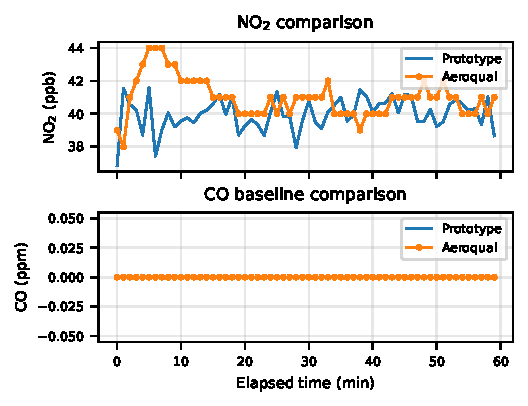
\includegraphics[width=0.96\columnwidth]{reference_comparison_compact_finalcal.pdf}
\caption{One-hour co-location comparison between the prototype and Aeroqual S500 after final zero-offset calibration. Top: NO\textsubscript{2} comparison in ppb. Bottom: CO clean-air baseline comparison in ppm.}
\label{fig:reference_comparison}
\end{figure}

\begin{figure}[H]
\centering
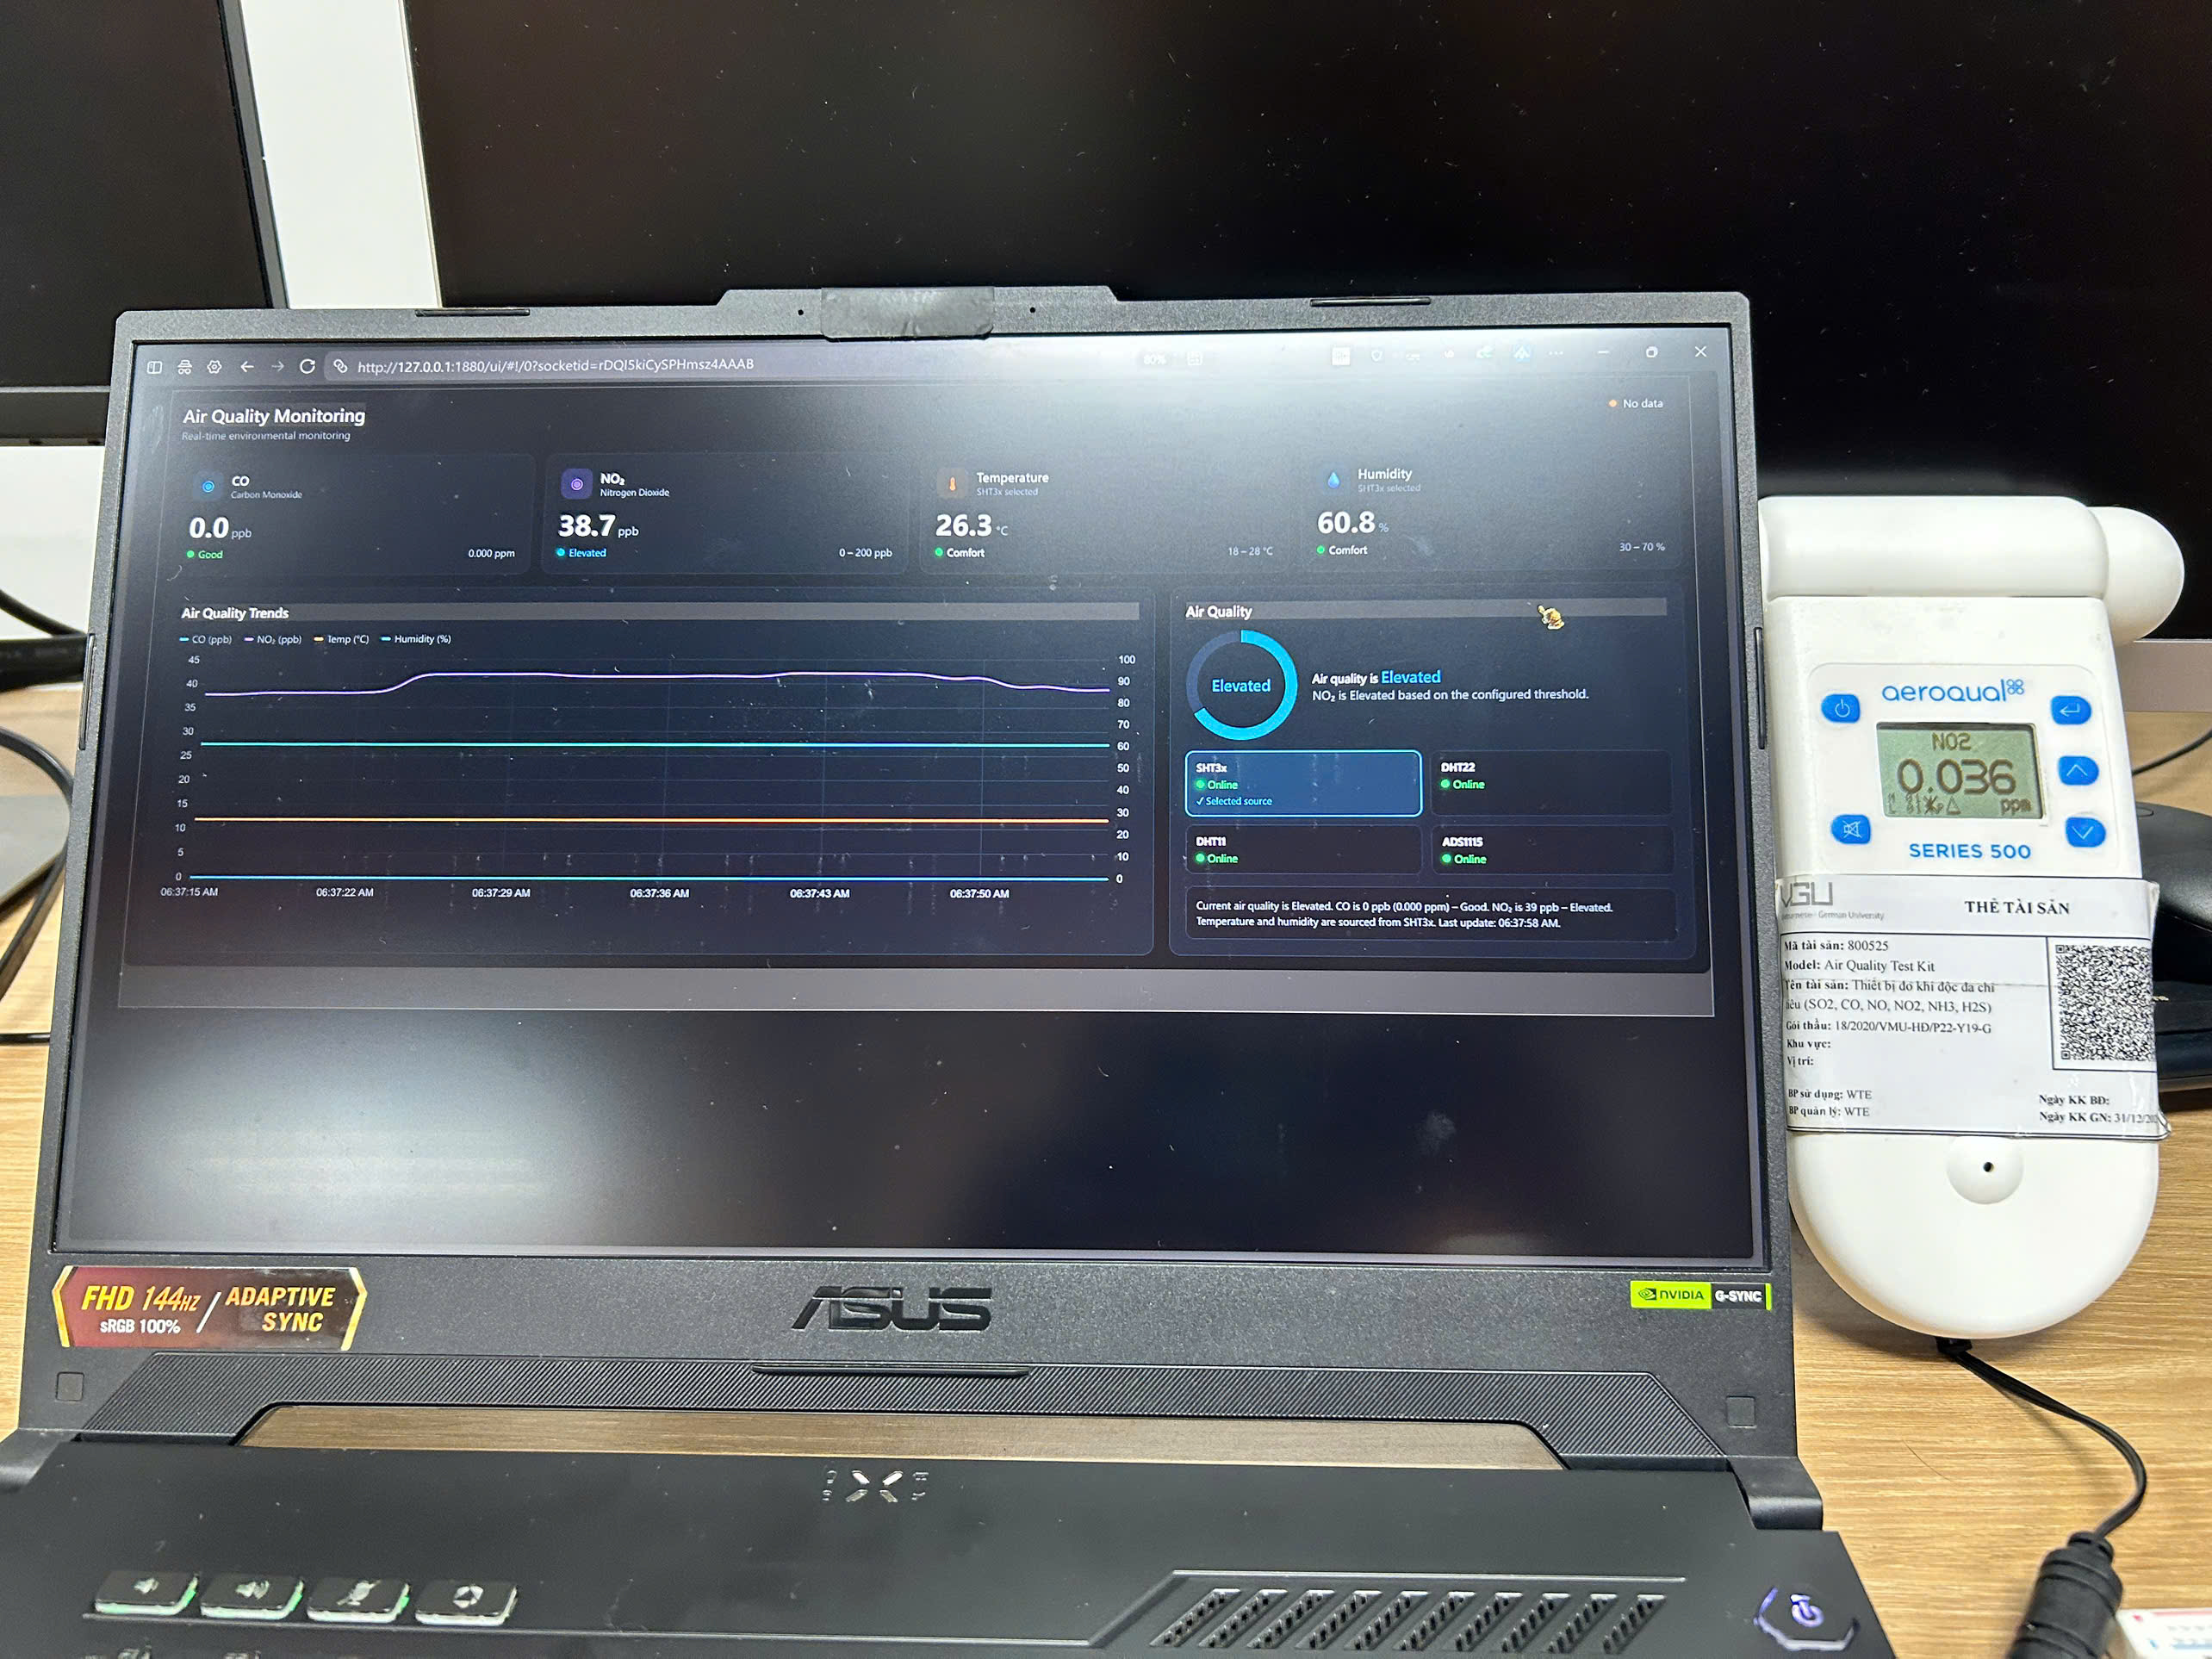
\includegraphics[width=0.96\columnwidth]{dashboard_aeroqual_reference_cropped.jpg}
\caption{Real-time co-location validation setup showing the Node-RED dashboard beside the Aeroqual S500 reference monitor. The dashboard displays the prototype's live CO, NO\textsubscript{2}, temperature, and humidity values, while the Aeroqual device provides the reference NO\textsubscript{2} reading used for manual comparison.}
\label{fig:dashboard_aeroqual_reference}
\end{figure}

\subsection{End-to-End Data Path}
After applying the calibration constants in firmware, the live dashboard renders post-calibration concentrations: CO near $0$~ppb (within the expected baseline noise) and NO\textsubscript{2} near $40$~ppb, matching the S500. The complete path from sensor read to dashboard update operates with end-to-end latency of under two seconds (sample period $1$~s, plus UART, MQTT, and rendering overhead). Under the dashboard thresholds in Table~\ref{tab:airquality_thresholds}, the CO channel remains in the Good range during this indoor run, while an NO\textsubscript{2} value near 40~ppb corresponds to the Elevated range. The flagged-atmosphere indicator therefore reports the worse gas-channel status rather than a generic or arbitrary \textit{Good} label.

\subsection{Security Outcome}
With TLS enabled, packet captures confirm that the JSON payload is unreadable on the wire. Plaintext clients are refused by the broker, and TLS clients without the trusted CA fail certificate verification. The gateway-to-broker hop therefore provides confidentiality and server authentication. The dashboard-to-broker hop is similarly TLS-secured. The pseudo-attack benchmark in Table~\ref{tab:tls_benchmark} further confirmed the expected enforcement of TLS handshake verification, MQTT username/password authentication, and topic-level authorization. The two inconclusive message-content checks are attributed to concurrent live telemetry on the same topic during a limited laboratory access window, not to an observed bypass of the TLS or ACL configuration.

\section{Discussion}

The applied offset calibration is suitable for a stable indoor environment where the dominant requirement is to remove the per-sensor electronic zero and produce readings consistent with a reference at the prevailing concentration. It is less suitable for environments with large dynamic range, where the unrefined sensitivity slope would dominate the error budget. For deployment in such environments, two complementary improvements are recommended.

First, a controlled-exposure step should be added to the calibration protocol. Briefly exposing the inlet to a measurable elevated CO concentration (e.g., a small combustion source under supervision, or co-locating outdoors near vehicle traffic for NO\textsubscript{2}) provides the second anchor point required for a two-point fit, yielding an empirical slope rather than the datasheet nominal.

Second, the residuals from the co-location window can be regressed against temperature and humidity to characterize cross-sensitivity. Alphasense publishes algorithm-based temperature compensation procedures for the B4 series; applying these would further improve accuracy across the temperature range encountered indoors over a day-night cycle.

A practical observation from the experiment is the warm-up behavior of the electrochemical channels. The preliminary calibration constants changed after extended operation because the ISB outputs continued settling after power-up. For this reason, the final deployed offsets were taken from the later one-hour co-location run rather than the earliest warm-up values. This behavior reinforces the need to allow sufficient warm-up time before calibration and to treat the reported zero offsets as session-specific values unless the sensor has been stabilized over a longer period.

\section{Conclusion}

A two-node low-cost air quality monitor was built and verified end to end. The sensor-to-gateway architecture isolates the analog signal chain from the wireless radio while providing a clean MQTT-over-TLS telemetry path to a live dashboard. Final calibration against the Aeroqual S500 produced session-specific electronic-zero offsets of $131.0$~mV for CO and $3.80$~mV for NO\textsubscript{2}, while retaining nominal sensitivity slopes because the co-location data contained only a single stable concentration region. The security verification (packet capture, handshake inspection, and negative tests) confirms that the telemetry hop is genuinely TLS-protected. The limitations of single-cluster co-location and manual reference logging are stated transparently, and a path to full two-point calibration with controlled exposure is identified as future work.


\section*{Acknowledgment}
The authors thank Mr. Tran Quang Nhu for guidance, and the ECE Communication Networks laboratory at Vietnamese--German University for access to the Aeroqual S500 reference instrument and the sensor inventory used in this work.

\begin{thebibliography}{00}
\bibitem{castell2017} N. Castell \textit{et al.}, ``Can commercial low-cost sensor platforms contribute to air quality monitoring and exposure estimates?,'' \textit{Environment International}, vol. 99, pp. 293--302, 2017.
\bibitem{mead2013} M. I. Mead \textit{et al.}, ``The use of electrochemical sensors for monitoring urban air quality in low-cost, high-density networks,'' \textit{Atmospheric Environment}, vol. 70, pp. 186--203, 2013.
\bibitem{alphasense_cob4} Alphasense Ltd., ``CO-B4 carbon monoxide sensor datasheet.''
\bibitem{alphasense_no2b43f} Alphasense Ltd., ``NO\textsubscript{2}-B43F nitrogen dioxide sensor datasheet.''
\bibitem{ti_ads1115} Texas Instruments, ``ADS1115 ultra-small, low-power, 16-bit, analog-to-digital converter,'' Datasheet SBAS444B.
\bibitem{sensirion_sht3x} Sensirion AG, ``SHT3x-DIS humidity and temperature sensor datasheet.''
\bibitem{espressif_idf} Espressif Systems, ``ESP-IDF Programming Guide,'' v6.0.
\bibitem{mqtt} OASIS, ``MQTT Version 5.0,'' OASIS Standard, 2019.
\bibitem{tls} E. Rescorla, ``The Transport Layer Security (TLS) Protocol Version 1.3,'' RFC 8446, 2018.
\end{thebibliography}

\end{document}